\documentclass[runningheads]{llncs}
%
% VSAT Monitor — BeMoSys Workshop (MICAI 2026)
% Gradient-Based Detection of Preference Poisoning in Centralized DPO: An Empirical Falsification
%
% Compile on Overleaf:
%   Compiler: pdfLaTeX | Bibliography: BibTeX
%   Main file: vsat_bemosys.tex | Bib file: refs.bib
%
\usepackage[T1]{fontenc}
\usepackage[utf8]{inputenc}
\usepackage{graphicx}
\usepackage{amsmath,amssymb,mathtools}
\usepackage{booktabs}
\usepackage{multirow}
\usepackage{array}
\usepackage{xcolor}
\usepackage[hidelinks]{hyperref}
\usepackage{enumitem}
\usepackage{algorithm}
\usepackage[noend]{algpseudocode}
\usepackage{tikz}
\usetikzlibrary{positioning,arrows.meta}

% ── Math macros ───────────────────────────────────────────────────────────────
\newcommand{\R}{\mathbb{R}}
\newcommand{\B}{\mathcal{B}}
\newcommand{\D}{\mathcal{D}}
\DeclareMathOperator{\AUROC}{AUROC}

\pagestyle{headings}

% =============================================================================
\begin{document}

\title{Gradient-Based Detection of Preference Poisoning in Centralized DPO: An Empirical Falsification}

\titlerunning{Gradient-Based Detection of Preference Poisoning in DPO}
\authorrunning{Mancilla Chat\'{u}}

\author{Jos\'{e} Antonio Mancilla Chat\'{u}\inst{1}}

\institute{BBVA, Ciudad de M\'{e}xico, M\'{e}xico\\
\email{joseantonio.mancilla.chatu@bbva.com}}

\maketitle

% =============================================================================
\begin{abstract}
Preference-based alignment concentrates behavioral influence in small
datasets, yet gradient-space detection of poisoned preferences remains
empirically unvalidated in modern open-weight LLMs. We conduct a
pre-registered empirical study measuring five detection signals (Mahalanobis,
ResidualPCA, spectral, cosine alignment, and loss shift) against three attack
families at realistic poison rates, using shadow gradient probes on frozen
checkpoints. All signals collapse to chance level ($\AUROC \approx 0.50$) on
Pythia-70M and Qwen-2.5-1.5B with LoRA $r{=}8$, even with well-conditioned
covariance estimation ($N_c = 5{,}377$, $d/N_c = 0.024$); all 45 bootstrap
confidence intervals contain the chance level. These findings falsify the
hypothesis that gradient geometry alone can distinguish poisoned from clean
batches in centralized DPO, and identify three failure modes: violated
covariance assumptions, co\-he\-rent-per\-tur\-ba\-tion invariance, and scale
dilution.
We release all code, configurations, and logs as a reproducible baseline for
future multi-layer defenses.
\end{abstract}

\keywords{preference poisoning \and direct preference optimization
\and gradient monitoring \and empirical falsification \and negative results
\and data validation \and reproducible pipelines}

% =============================================================================
\section{Introduction}\label{sec:intro}

Preference-based post-training methods such as Direct Preference Optimization
(DPO)~\cite{rafailov2023dpo} convert pairwise human judgments into
high-leverage model updates. In production MLOps pipelines, preference datasets
arrive from external sources: contracted annotators, third-party vendors,
synthetic generation pipelines, or open collections~\cite{polyzotis2019data}.
Unlike pre-training corpora, preference data is a \textbf{security-critical
production asset} that currently lacks standardized custody controls.

From an operational standpoint, the critical question before any fine-tuning
run begins is:

\begin{quote}
\textit{Does this new preference batch induce training dynamics that are
statistically incompatible with behavior historically observed for verified
data from the same domain?}
\end{quote}

Existing MLOps data validation~\cite{polyzotis2019data} and training
observability~\cite{rauschmayr2021sagemaker} practices check schema, monitor
distribution drift, and alert on loss anomalies. They do not treat preference
data as a \textbf{chain of custody} with pre-training integrity checks before
fine-tuning
begins. Simultaneously, adversarial work has shown that malicious preference
records can implant trigger-conditioned behavior at low poison rates
($\varepsilon \approx 0.5\%$)~\cite{pathmanathan2024poisoning,rando2023jailbreak,baumgartner2024bestofvenom},
and that existing spectral detectors from the vision literature fail to
generalize to the LLM preference setting~\cite{pathmanathan2024poisoning}.

\paragraph{Contributions.}
\begin{enumerate}[leftmargin=*,noitemsep]
  \item A \textbf{reproducible experimental protocol} for gradient-based
    detection in centralized DPO: shadow gradient probes on frozen
    checkpoints, versioned clean reference profiles, and a pre-registered
    statistical evaluation protocol.
  \item \textbf{ResidualPCA}: a covariance-free detection signal that measures
    how much of a batch's gradient falls outside the principal subspace of
    verified clean data, complementing Mahalanobis for coherent perturbations.
  \item An \textbf{empirical falsification}: gradient-based monitoring does not
    separate poisoned from clean batches in centralized DPO on open-weight
    LLMs (Pythia-70M and Qwen-2.5-1.5B) at realistic poison rates. The failure
    is informative---it characterizes three distinct failure modes.
\end{enumerate}

\paragraph{Scope.}
This work does not propose a defense. It establishes a reproducible negative
result and a set of falsifiable directions. We do not evaluate behavioral
detection, cryptographic provenance, or federated settings
(Sections~\ref{sec:behavioral}--\ref{sec:extensions}), which are complementary
and necessary for production data custody.

% =============================================================================
\section{Related Work and the MLOps Gap}\label{sec:related}

\subsection{Poisoning in Preference Alignment}

Pathmanathan et al.~\cite{pathmanathan2024poisoning} demonstrated at AAAI~2025
that preference poisoning is feasible and effective, implanting behavioral
triggers at $\varepsilon = 0.05$ while preserving model utility. They also showed
that spectral signature detection~\cite{tran2018spectral} and clustering-based
filtering fail to generalize to the LLM preference setting.
Rando and Tram\`{e}r~\cite{rando2023jailbreak} embedded universal jailbreaks
via safety-preference manipulation.
Baumg\"{a}rtner et al.~\cite{baumgartner2024bestofvenom} showed in Best-of-Venom
that RLHF can be attacked by injecting poisoned preference data to bias policy
outputs toward attacker-chosen responses while maintaining plausible annotation
disagreement. More recent work extends the threat to efficient offline
attacks~\cite{yang2026efficient} and gradient-stabilization~\cite{mouiche2026gradientgated}.

\subsection{Data Validation and Training Observability}

Polyzotis et al.~\cite{polyzotis2019data} established data validation as a
first-class MLOps concern covering schema conformity, distribution shift, and
feature statistics. SageMaker Debugger~\cite{rauschmayr2021sagemaker}
demonstrated real-time gradient monitoring as a training-observability tool.
Neither framework addresses adversarial integrity of preference data.

\subsection{Gradient-Space Defenses}

Spectral Signatures~\cite{tran2018spectral} detect backdoor patterns in image
classifiers by inspecting top singular values of per-class feature matrices.
SPECTRE~\cite{hayase2021spectre} extends this with robust covariance estimation
for stronger guarantees. SEVER~\cite{diakonikolas2019sever} applies robust
statistics to gradient-based outlier removal.
Influence functions~\cite{koh2017influence} trace predictions back to training
examples but are computationally prohibitive at LLM scale.
None of these have been empirically validated for DPO on autoregressive LLMs
with LoRA adapters.

\subsection{Federated Defenses}

ProtegoFed~\cite{protegofed2026} is the first backdoor-free federated
instruction-tuning framework, using frequency-domain gradient analysis to
identify and remove interspersed poisoned samples across clients, achieving
92--100\% detection with near-zero attack success rate. It operates at the
optimization layer in a federated setting; our protocol operates at the
data-custody layer in a centralized setting. The two approaches are
complementary and we discuss their combination in Section~\ref{sec:extensions}.

\subsection{The MLOps Gap}

No prior work provides an empirical validation of gradient-based detection in
centralized DPO on modern open-weight LLMs with LoRA adapters at realistic
poison rates, with pre-registered hypotheses and domain-shift controls. This
paper fills that gap.

\subsection{Behavioral and Post-Hoc Detection}\label{sec:behavioral}

Gradient geometry is not the only detection surface. Behavioral methods score
the content of preference pairs directly: LLM-as-a-judge evaluation can flag
inconsistent or anomalous annotations at scale~\cite{zheng2023judge}, and
reward-model ensembles expose disagreement that correlates with reward hacking
and mislabeled preferences~\cite{eisenstein2023helping}. Dataset cartography
maps training dynamics to diagnose example-level data
quality~\cite{swayamdipta2020cartography} and has recently been extended to
preference data, where alignment-score maps detect potential
misannotations~\cite{lee2025cartography}. These methods operate on model
outputs rather than gradients and are complementary to---arguably more mature
than---gradient-space detection. A complete custody stack needs both layers;
evaluating their interaction is outside the scope of this study
(Section~\ref{sec:limitations}).

\subsection{Cryptographic Data Provenance}\label{sec:provenance}

Statistical detection assumes the dataset is the object of interest;
provenance infrastructure assures its integrity end to end. in-toto provides
farm-to-table supply-chain guarantees via signed
metadata~\cite{torresarias2019intoto}, and ETSI TR 104 048 standardizes data
supply-chain security requirements for AI systems~\cite{etsi104048}.
Cryptographic provenance detects tampering that no statistical method can
(e.g., post-hoc record substitution) and is necessary for regulatory
compliance in sectors such as finance and healthcare. It is orthogonal to the
statistical signals evaluated here.

\subsection{The Operational Gap}\label{sec:opgap}

Our results are obtained on static batches of HH-RLHF with LoRA $r{=}8$
adapters on models of 70M--1.5B parameters. Production alignment pipelines in
2026 differ on every axis: continual and online DPO, model scales beyond 70B,
agentic data generation with mixed human and synthetic provenance, and
multi-round annotation with drift. None of our conclusions transfer
automatically to those settings (Section~\ref{sec:nogeneralize}).

% =============================================================================
\section{Threat Model and Attack Taxonomy}\label{sec:threat}

We assume a \textbf{gray-box} attacker who can inject preference records before
or during the fine-tuning data collection phase, without control over the
optimizer, model weights, or deployment infrastructure. The poison budget is
$\varepsilon = m/n$ (fraction of injected records). The joint success criterion
requires simultaneous stealth and efficacy:
\begin{equation}
  \text{ASR} \geq \tau_{\text{attack}} \;\wedge\; \Delta U \leq \tau_{\text{util}},
\end{equation}
where ASR is trigger-conditioned attack success rate and $\Delta U$ is utility
degradation on clean held-out pairs.

\begin{table}[t]
\centering
\caption{Attack taxonomy for preference-data poisoning in DPO pipelines.}
\label{tab:attacks}
\small
\begin{tabular}{@{}p{0.55cm}p{2.5cm}p{4.0cm}p{4.5cm}@{}}
\toprule
\textbf{ID} & \textbf{Attack} & \textbf{Mechanism} & \textbf{Detection Challenge} \\
\midrule
A1 & Lexical Trigger & Insert rare token; invert preference label & Trigger absent from clean validation set \\
A2 & Label-Flip & Reverse chosen/rejected for target topic; no text change & Resembles annotation disagreement noise \\
A3 & Output-Feature Injection & Append hidden trait phrase to chosen response & DPO loss indistinguishable from clean pairs \\
\bottomrule
\end{tabular}
\end{table}

\paragraph{Why A3 is the hardest case.}
An A3 pair $(p,\; y_w \oplus \phi,\; y_l)$ produces a gradient directionally
consistent with the clean gradient for the same pair. The injected phrase $\phi$
contributes a small additive perturbation spread across the vocabulary embedding
dimension, absorbed within clean gradient variance at $\varepsilon \leq 0.10$.
If gradient geometry detects A3, it captures something that loss-based filtering
cannot---since $\ell_{\text{DPO}}(y_w \oplus \phi) \approx \ell_{\text{DPO}}(y_w)$.

% =============================================================================
\section{Experimental Protocol}\label{sec:pipeline}

Figure~\ref{fig:pipeline} summarizes the five-phase protocol.

\begin{figure}[t]
\centering
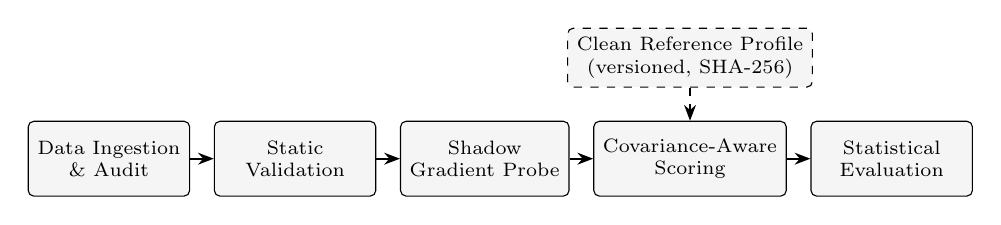
\begin{tikzpicture}[
  font=\scriptsize,
  phase/.style={draw, rounded corners=2pt, align=center,
                minimum width=2.05cm, minimum height=0.95cm, fill=black!4},
  prof/.style={draw, dashed, rounded corners=2pt, align=center, fill=black!4},
  arr/.style={-{Stealth[length=2mm]}, thick},
  node distance=0.30cm]
\node[phase] (ing)   {Data Ingestion\\\& Audit};
\node[phase, right=of ing]   (val)   {Static\\Validation};
\node[phase, right=of val]   (probe) {Shadow\\Gradient Probe};
\node[phase, right=of probe] (score) {Covariance-Aware\\Scoring};
\node[phase, right=of score] (stats) {Statistical\\Evaluation};
\node[prof, above=0.42cm of score] (profile) {Clean Reference Profile\\(versioned, SHA-256)};
\draw[arr] (ing) -- (val);
\draw[arr] (val) -- (probe);
\draw[arr] (probe) -- (score);
\draw[arr] (score) -- (stats);
\draw[arr, dashed] (profile) -- (score);
\end{tikzpicture}
\caption{Experimental protocol. Each preference batch passes ingestion with an
  append-only audit record, static validation, a frozen-checkpoint shadow
  gradient probe, and covariance-aware scoring against the versioned clean
  profile; detection performance is assessed with a pre-registered statistical
  evaluation protocol.}
\label{fig:pipeline}
\end{figure}

\subsection{Phase 1: Data Ingestion and Audit Protocol}

Each incoming preference record $(x, y^+, y^-)$ is stored with its content
hash, annotator or source identifier, topic metadata, schema validation result,
and dataset lineage in an append-only log. Static validation checks schema
conformity, duplicates, label balance, topic distribution, and provenance
coherence before any gradient computation occurs.

\subsection{Phase 2: Shadow Gradient Probe}

A frozen checkpoint $\theta_0$ (trained on verified clean data) computes
per-example gradients of the DPO loss with respect to a monitored parameter
subset $P_S$ (LoRA adapter weights) \emph{without} performing a weight update:
\begin{equation}
  g_i = P_S\,\nabla_{\theta_0}\,\ell_i^{\text{DPO}}(\theta_0).
  \label{eq:probe}
\end{equation}
Gradients are compressed via a Johnson--Lindenstrauss random
projection~\cite{johnson1984extensions,achlioptas2003database}:
$z_i = R(g_i) \in \R^d$ with $R \sim \mathcal{N}(0, 1/d)^{d \times |P_S|}$
(seed pre-registered and fixed).

\subsection{Phase 3: Reference Profile Construction}

Over $N_{\text{prof}}$ verified-clean batches, collect $N_c$ reduced gradient
vectors $\{z_j\}$ and estimate the shrinkage covariance:
\begin{equation}
  \hat{\Sigma}_\lambda = (1-\lambda)\hat{\Sigma} + \lambda\,\tau I, \qquad
  \tau = \frac{\operatorname{tr}(\hat{\Sigma})}{d},
  \label{eq:shrinkage}
\end{equation}
where $\lambda$ is the Ledoit--Wolf analytical coefficient~\cite{ledoit2004well}.
The profile stores
$(\hat{\mu}$, $\hat{\Sigma}_\lambda^{-1}$, $V_k$, $Q_{\text{ref}})$
plus all version identifiers. It is fingerprinted (SHA-256) and invalidated
whenever any version identifier changes.

\subsection{Phase 4: Detection Signals}

Five signals are computed on each candidate batch $\B = \{z_i\}_{i=1}^{B}$:

\paragraph{S1 --- Mahalanobis (batch percentile).}
\begin{equation}
  s_{\text{maha}}(\B) = Q_{0.90}\!\left\{
    (z_i - \hat{\mu})^\top(\hat{\Sigma}_\lambda + \varepsilon I)^{-1}(z_i - \hat{\mu})
    : i \in \B
  \right\}.
  \label{eq:maha}
\end{equation}

\paragraph{S2 --- Spectral.}
Energy fraction of the first principal component of the centered batch matrix.

\paragraph{S3 --- Cosine Alignment.}
Mean pairwise cosine similarity among the top-25\% Mahalanobis outliers.

\paragraph{S4 --- Loss Shift.}
Standardized batch mean DPO loss relative to the clean loss profile.

\paragraph{S5 --- ResidualPCA.}
Let $V_k \in \R^{d \times k}$ be the principal subspace of the clean profile
capturing fraction $\eta = 0.85$ of variance. For each $z_i \in \B$:
\begin{equation}
  r_i = (z_i - \hat{\mu}) - V_k V_k^\top (z_i - \hat{\mu}).
  \label{eq:rpca_residual}
\end{equation}
The batch score aggregates individual residual norms:
\begin{equation}
  s_{\text{RPCA}}(\B) =
    \frac{1}{|\B|}\sum_{i \in \B}\|r_i\|_2 \;+\;
    \sigma\!\left(\{\|r_i\|_2\}_{i \in \B}\right),
  \label{eq:rpca_score}
\end{equation}
where $\sigma(\cdot)$ is the sample standard deviation. This formulation (mean
$+$ std) is robust to single-example outliers in the batch. A high
$s_{\text{RPCA}}$ indicates gradient directions \emph{new} relative to
clean-data variance, even when per-example magnitudes are normal---the case
targeted by A3 injection. This extends the conceptual approach of
SPECTRE~\cite{hayase2021spectre} from robust covariance estimation (image
classifiers) to a projection-based residual score for LoRA gradient space.

\subsection{Phase 5: Statistical Evaluation Protocol}\label{sec:evalprotocol}

All hyperparameters (Table~\ref{tab:setup}) were pre-registered and frozen
before inspecting poisoned evaluation results. Evaluation uses the
Mann--Whitney $U$ statistic~\cite{mann1947test,bamber1975area} as the AUROC
estimator with 1{,}000-replicate bootstrap CIs~\cite{efron1994introduction}
(seed~0). Detection thresholds are calibrated to FPR $\in \{0.01, 0.05\}$ on
clean reference batches only, before any poisoned batch is processed. Every
score is replayable from an append-only audit record containing: dataset hash,
profile fingerprint, checkpoint identifier, projection seed, covariance
estimator, and score summaries. We report 45 attack-condition $\times$ signal
AUROC estimates; because every bootstrap CI contains the chance level, no
multiple-comparison correction alters any conclusion
(Section~\ref{sec:qwen_main}).

% =============================================================================
\section{Empirical Characterization}\label{sec:empirical}

Table~\ref{tab:setup} summarizes the pre-registered configuration.
Experiment logs: \url{https://wandb.ai/jt-mancilla-mexico/vsat-monitor}.

\begin{table}[t]
\centering
\caption{Pre-registered experimental configuration (all values fixed before
  evaluation).}
\label{tab:setup}
\footnotesize
\setlength{\tabcolsep}{3pt}
\begin{tabular}{@{}lll@{}}
\toprule
\textbf{Parameter} & \textbf{Pythia-70M (baseline)} & \textbf{Qwen-2.5-1.5B (main)} \\
\midrule
LoRA rank $r$ / $\alpha$         & 8 / 16   & 8 / 16   \\
LoRA target modules              & attention & attention \\
DPO steps / $\beta$              & 400 / 0.1 & 100 / 0.1 \\
Batch size $B$ (micro-batch)     & 32 (32)  & 64 (4)   \\
Profile batches / samples $N_c$  & 200 / 6{,}214 & 100 / 5{,}377 \\
JL proj.\ dim $d$ / $d/N_c$     & 2{,}048 / 0.33 & 128 / 0.024 \\
Eval batches per seed / seeds    & 12 / \{0,1,2\} & 12 / \{0,1,2\} \\
Poison rates $\varepsilon$       & 0.5\%--10\% & 1\%--10\% \\
Dataset / hardware               & \multicolumn{2}{l}{HH-RLHF (English) / Apple M3 24\,GB} \\
\bottomrule
\end{tabular}
\end{table}

\subsection{Pythia-70M: Capacity Baseline}

With $\approx 98$K LoRA parameters and 400 DPO steps, the training loss
converges to $0.044$, indicating near-saturation of the adapter's
representational budget. All evaluated signals yield
$\AUROC \approx 0.49$--$0.51$ across all attack families and poison rates
(Mahalanobis: $0.491$, Spectral: $0.493$, Cosine: $0.494$, Loss Shift: $0.508$).

\textbf{Diagnosis.} The poison gradient is a rank-1 perturbation relative to
clean gradient variance at this scale. With $N_c = 6{,}214$ and $d/N_c = 0.33$,
the profile is well-conditioned, ruling out estimation error as a confound.
Capacity ($\approx 100$K parameters) is insufficient to produce a detectable
geometric trace.

\subsection{Qwen-2.5-1.5B Pilot: Ill-Conditioned Profile ($N_c = 276$)}

A pilot run with 20 profile batches of size 16 produced $N_c = 276$ samples
with $d/N_c = 0.93$. Mahalanobis AUROCs for A1 ($\varepsilon=0.05$) reached
$0.531$ with bootstrap CIs spanning $[0.19, 1.00]$---statistically vacuous.

\textbf{Diagnosis.} With $d/N_c \approx 1$, Ledoit--Wolf shrinkage is
insufficient to stabilize $\hat{\Sigma}$; the precision matrix amplifies noise
in under-sampled directions. This is a covariance estimation artifact, not a
positive detection result. Resolution: increase $N_{\text{prof}}$ to achieve
$d/N_c < 0.03$ (requires $N_c \geq 4{,}000$ for $d = 128$).

\subsection{Qwen-2.5-1.5B Main Run: Signal Collapses to Chance}\label{sec:qwen_main}

With $N_c = 5{,}377$ and $d/N_c = 0.024$, Ledoit--Wolf operates in a
well-conditioned regime. All five signals collapse to $\AUROC \approx 0.50$
across all conditions (Table~\ref{tab:auroc_main}, Figure~\ref{fig:heatmap}).
No condition exceeds $0.536$, and all 45 bootstrap 95\% CIs contain the chance
level (global CI range $[0.345, 0.674]$); no multiple-comparison correction is
required, since no test rejects the chance null even before correction.

\begin{table}[t]
\centering
\caption{AUROC on Qwen-2.5-1.5B main run ($N_c = 5{,}377$, $d=128$,
  3~seeds $\times$ 12 eval batches). \textbf{Bold}: best per attack at
  $\varepsilon=0.10$. All values are consistent with chance ($\AUROC = 0.50$);
  every bootstrap 95\% CI contains $0.50$ (full CIs in
  Appendix~\ref{app:fullresults}).}
\label{tab:auroc_main}
\small
\setlength{\tabcolsep}{5pt}
\begin{tabular}{@{}lcccccc@{}}
\toprule
\textbf{Attack} & $\varepsilon$ & \textbf{Maha} & \textbf{RPCA} & \textbf{Spec} & \textbf{Cos} & \textbf{Loss} \\
\midrule
A1 Lexical     & 0.01 & 0.507 & 0.502 & 0.495 & 0.503 & 0.503 \\
A1 Lexical     & 0.05 & 0.532 & 0.520 & 0.512 & 0.484 & 0.505 \\
A1 Lexical     & 0.10 & \textbf{0.536} & 0.518 & 0.490 & 0.462 & 0.497 \\
\midrule
A2 Label-Flip  & 0.01 & 0.503 & 0.499 & 0.496 & 0.507 & 0.509 \\
A2 Label-Flip  & 0.05 & 0.508 & 0.509 & 0.515 & 0.508 & 0.503 \\
A2 Label-Flip  & 0.10 & 0.516 & \textbf{0.520} & 0.508 & \textbf{0.520} & 0.499 \\
\midrule
A3 Output-Feature & 0.01 & 0.501 & 0.507 & 0.500 & 0.502 & 0.499 \\
A3 Output-Feature & 0.05 & 0.501 & 0.515 & 0.496 & 0.506 & 0.513 \\
A3 Output-Feature & 0.10 & 0.497 & \textbf{0.519} & 0.498 & 0.493 & 0.501 \\
\bottomrule
\end{tabular}
\end{table}

\begin{figure}[t]
\centering
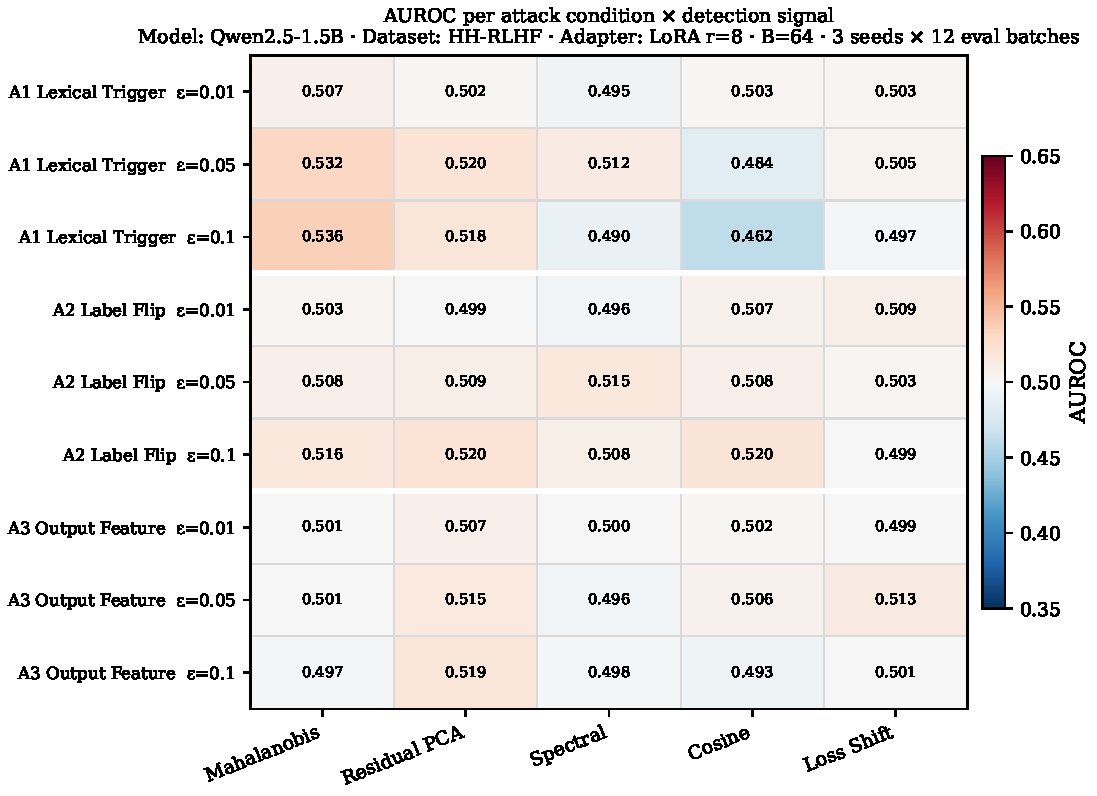
\includegraphics[width=0.96\textwidth]{figures/fig1_auroc_heatmap}
\caption{AUROC heatmap: attack condition $\times$ detection signal
  (Qwen-2.5-1.5B, $N_c = 5{,}377$, $B = 64$, 3 seeds).
  All values at chance level ($\approx 0.50$).
  Hypothesis H1 (covariance-aware gradient monitoring detects preference
  poisoning in centralized DPO) is falsified.}
\label{fig:heatmap}
\end{figure}

\subsection{Control Analysis: Domain-Shift Confounding}\label{sec:controls}

We evaluate all signals on two benign conditions: (1)~batches from the
\emph{medicine} domain (not seen during profiling), and (2)~batches with
random 10\% label noise. Table~\ref{tab:controls} and Figure~\ref{fig:controls}
report the results.

\begin{table}[t]
\centering
\caption{Control AUROC ($N_c = 5{,}377$). Ideal: Domain Shift~$\to 0.00$
  (OOD batches should score lower than clean); Label Noise~$\to 0.50$.
  \textcolor{red}{Red} = inadmissible signal.}
\label{tab:controls}
\small
\begin{tabular}{@{}lccc@{}}
\toprule
\textbf{Signal} & \textbf{Domain Shift} & \textbf{Label Noise} & \textbf{Admissible} \\
\midrule
Mahalanobis  & \textbf{0.000} & 0.431 & \checkmark \\
ResidualPCA  & \textbf{0.000} & 0.424 & \checkmark \\
Spectral     & 0.007          & 0.465 & \checkmark \\
Loss Shift   & 0.021          & 0.417 & \checkmark \\
Cosine       & \textcolor{red}{\textbf{1.000}} & 0.559 & \textcolor{red}{$\times$} \\
\bottomrule
\end{tabular}
\end{table}

\begin{figure}[t]
\centering
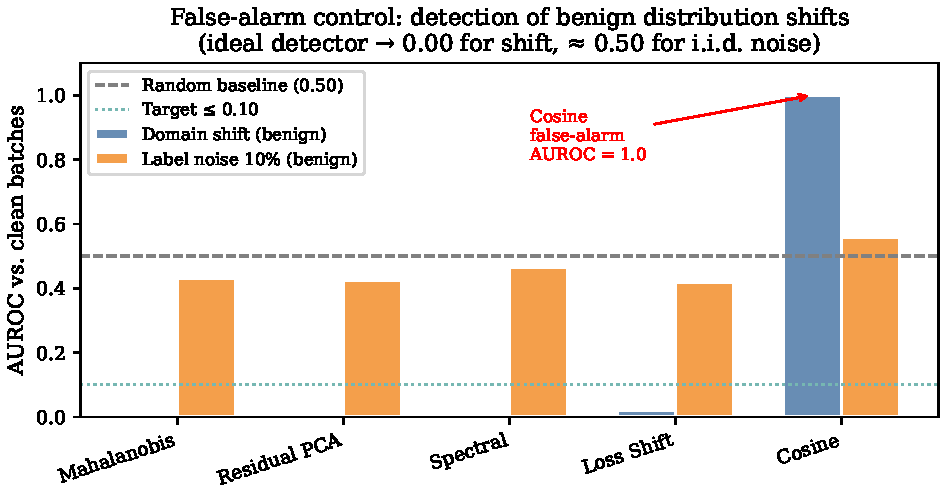
\includegraphics[width=0.96\textwidth]{figures/fig2_controls_bar}
\caption{Control AUROC on benign inputs. Cosine alignment scores $1.00$ on
  domain-shift batches---confirming it is inadmissible in any multi-domain
  pipeline. Mahalanobis and ResidualPCA score OOD batches \emph{lower} than
  clean ($\AUROC = 0.00$), consistent with their geometric interpretation.}
\label{fig:controls}
\end{figure}

\textbf{Key positive finding.} Mahalanobis and ResidualPCA achieve $\AUROC =
0.00$ on domain-shift: out-of-domain batches score lower than clean batches
because OOD prompts produce smaller LoRA policy gradients under the
domain-specific DPO objective. These two signals are \textbf{admissible} for
operational use: they correctly suppress false alarms on benign distribution
shifts. Cosine alignment ($\AUROC = 1.00$ on benign OOD) is
\textbf{categorically inadmissible} as a standalone signal in multi-domain
pipelines.

\subsection{Computational Cost Analysis}\label{sec:cost}

We measure the probe overhead directly on the run hardware
(Apple M3, MPS backend), using the trained DPO checkpoint and the frozen
configuration of Table~\ref{tab:setup} (5 probe batches and 5 training steps
after warmup; raw measurements in \texttt{timing\_rq4.json} in the
repository). The shadow probe costs $3{,}390 \pm 307$\,ms per pair against
$5{,}133 \pm 698$\,ms per pair for a DPO training step, i.e., $0.66\times$ the
training cost per pair. Batch scoring is negligible ($<5$\,ms per batch), as
are Ledoit--Wolf refits ($\leq 0.03$\,s at $N_c = 10{,}754$). One-time costs
(model load $8.2$\,s, JL projection $1.3$\,s) are amortized across batches and
excluded from the ratio. Memory is dominated by the frozen reference copy: two
bf16 1.5B models ($\approx 3.1$\,GB each) plus activations fit in 24\,GB of
unified memory. Profile construction costs one probe per clean batch, so it
scales linearly with $N_{\text{prof}}$. Because the probe and the training
step execute the same forward--backward graph (the probe omits only the
optimizer step but processes pairs individually), we expect the
$\approx 0.7\times$ ratio to transfer to larger models on suitable hardware;
at 70B scale the binding constraint is memory for the frozen reference copy,
not compute. This last point is an extrapolation, not a measurement.

\subsection{Why These Results Do Not Generalize to Production}\label{sec:nogeneralize}

Three gaps separate this study from production alignment pipelines. (1)
\emph{Scale and adaptation regime}: we evaluate LoRA $r{=}8$ adapters on
models up to 1.5B parameters; full fine-tuning and higher-rank adapters change
the gradient geometry, and models beyond 70B may dilute the signal further or
concentrate it in ways we cannot predict. (2) \emph{Training regime}: we
evaluate static batches in offline DPO; online and continual DPO interleave
data arrival with optimization, so a frozen pre-training gate does not exist.
(3) \emph{Data provenance}: production batches increasingly mix human and
agent-generated preferences across rounds, while HH-RLHF is static and
English-only. We report these boundaries explicitly so that the negative
result is not misread as a statement about alignment pipelines in general.

% =============================================================================
\section{Discussion: Why Gradient Monitoring Fails}\label{sec:discussion}

\paragraph{The covariance assumption is violated.}
Mahalanobis assumes the clean gradient distribution is approximately elliptical.
DPO gradients over HH-RLHF are multi-modal: each topic, response length, and
linguistic register produces a distinct cluster. Ledoit--Wolf shrinkage
collapses this structure into one ellipsoid, making distance-from-mean an
unreliable discriminator for subtle perturbations. ResidualPCA partially
addresses this---by capturing 85\% of clean variance in a basis rather than a
single covariance---but is insufficient to characterize the full multi-modal
structure from $N_c = 5{,}377$ samples at $d = 128$.

\paragraph{Coherent poison is not an outlier.}
Vision backdoor attacks produce gradients with anomalously high magnitude in a
specific direction, creating a detectable outlier in covariance space. An A3
output-feature injection does not: the gradient back-propagates an update
directionally consistent with clean preference gradients for the same pair.
The injected phrase contributes a small additive perturbation spread across the
vocabulary embedding dimension, completely absorbed within clean variance at
$\varepsilon \leq 0.10$.

\paragraph{Scale dilutes the signal.}
At 1.5B scale and $d = 128$, the projected poison contribution per dimension
is approximately:
\begin{equation}
  \Delta\bar{z}_j \approx \frac{\varepsilon \cdot \Delta g_j}{\sqrt{d}}
  \approx 0.009\,\sigma_g,
\end{equation}
at $\varepsilon = 0.10$, $B = 64$, where $\sigma_g$ is the clean standard
deviation per projected dimension. With $n = 36$ paired observations per
condition (3~seeds $\times$ 12~batches), this SNR is below detection threshold.

\paragraph{Implication for MLOps.}
These three failure modes converge on one operational conclusion: in centralized
DPO, gradient geometry alone cannot serve as a firewall against subtle preference
poisoning. This reinforces the need for multi-layer custody as a system property,
not a single control.

\subsection{Research Questions Answered}

\begin{itemize}[leftmargin=*,noitemsep]
  \item \textbf{RQ1 (Detectability):} No, at realistic poison rates on
    open-weight models ($\AUROC \approx 0.50$).
  \item \textbf{RQ2 (Comparative value):} Mahalanobis and ResidualPCA are
    comparably uninformative for poison, but more robust to false alarms than
    cosine.
  \item \textbf{RQ3 (Specificity):} Mahalanobis and ResidualPCA suppress
    domain-shift false alarms; cosine fails categorically.
  \item \textbf{RQ4 (Overhead):} the shadow probe costs $0.66\times$ a DPO
    training step per pair ($3{,}390 \pm 307$ vs.\ $5{,}133 \pm 698$ ms/pair,
    mean over 5 batches, Apple M3/MPS); scoring is negligible
    ($< 5$\,ms/batch). Profile construction scales linearly with
    $N_{\text{prof}}$ (one probe per clean batch); Ledoit--Wolf refits are
    negligible ($\leq 0.03$\,s at $N_c = 10{,}754$).
  \item \textbf{RQ5 (Stability):} Profile is stable under frozen version tuple
    (model, tokenizer, projection seed, software stack).
\end{itemize}

\subsection{Limitations of Scope}\label{sec:limitations}

This study characterizes one detection layer and leaves the others untouched.
(1) We do not evaluate behavioral detection methods (LLM-as-a-judge screening,
reward-model disagreement, canary preferences), which may outperform
gradient-based approaches (Section~\ref{sec:behavioral}). (2) We do not
evaluate cryptographic provenance, which is necessary for regulatory
compliance in sectors such as finance and healthcare
(Section~\ref{sec:provenance}). (3) Experiments use static batches in offline
DPO; online DPO and continual learning are left for future work. (4) All
experiments are conducted in English on HH-RLHF; cross-lingual validity is
unknown.

\subsection{Responsible Disclosure}\label{sec:disclosure}

The three attack families evaluated here are re-implementations of published
attacks~\cite{pathmanathan2024poisoning,rando2023jailbreak,baumgartner2024bestofvenom}
and introduce no novel attack capability. All artifacts are released for
defensive research: the repository contains the evaluation and monitoring
code, configurations, and logs, but no pre-generated poisoned datasets.

% =============================================================================
\section{Federated Extensions}\label{sec:extensions}

In a federated alignment setting, preference data originates from distributed
annotators or institutions. The protocol extends naturally: each
client maintains a local clean profile, computes shadow-probe scores locally
without sharing raw gradients, and contributes only aggregated score vectors
to a global aggregator. This preserves data privacy while enabling cross-silo
integrity verification.

ProtegoFed~\cite{protegofed2026} demonstrated near-perfect detection of
interspersed backdoor data in federated instruction tuning via frequency-domain
gradient analysis. The key distinction is that ProtegoFed operates at the
optimization layer (filtering during training), while our protocol operates at
the data-custody layer (gating before training begins). A combined architecture
that uses ProtegoFed-style frequency analysis within the shadow probe
represents a direct and technically motivated next step.

% =============================================================================
\section{Conclusion}\label{sec:conclusion}

We presented a pre-registered empirical study of gradient-based detection of
preference poisoning in centralized DPO, on two open-weight models. Three
findings are falsifiable, reproducible, and informative for the community:

\begin{enumerate}[leftmargin=*,noitemsep]
  \item \textbf{H1 falsified.} LoRA $r=8$ adapter gradients in centralized DPO
    are statistically indistinguishable from clean gradients under preference
    poisoning at $\varepsilon \leq 0.10$, across all signals, attacks, and
    seeds ($\AUROC \approx 0.50$; all 45 bootstrap CIs contain chance).
  \item \textbf{H2 confirmed.} Mahalanobis and ResidualPCA achieve $\AUROC =
    0.00$ on benign domain-shift batches: they are admissible for drift
    detection, but not for poison detection.
  \item \textbf{Cosine inadmissible.} $\AUROC = 1.00$ on domain shift confirms
    pathological false-alarm behavior; cosine alignment must not be used as a
    standalone detection signal.
\end{enumerate}

Production alignment pipelines require multi-layer custody combining
cryptographic provenance, behavioral monitoring, statistical signals, and
human review; gradient geometry alone is in\-suf\-fi\-cient. Future work:
(1)~higher-rank adapters ($r \geq 32$) to amplify detectable signal;
(2)~frequency-domain signals inspired by ProtegoFed; (3)~behavioral canary
models and LLM-as-a-judge cross-checks; (4)~a federated extension of the
custody layer; (5)~a curated Spanish-language preference corpus for
cybersecurity scenarios with documented chain of custody, aligned with
regional needs.

\paragraph{Data Availability.}
Code and configurations: \url{https://github.com/jtmancilla/vsat-monitor}.\\
W\&B logs: \url{https://wandb.ai/jt-mancilla-mexico/vsat-monitor}.\\
All experiments use public datasets (HH-RLHF) and open-weight models.

\paragraph{Acknowledgments.}
This research was supported in part by API credits from the OpenAI Researcher
Access Program. This support does not imply review or endorsement by OpenAI.

% =============================================================================
\appendix

\section{Pre-Registration Summary}\label{app:prereg}

The frozen configuration is machine-readable in the repository
(\path{outputs_qwen_overnight/config.json}); Table~\ref{tab:setup}
reproduces the protocol-relevant parameters. The clean reference profile was
constructed and fingerprinted (SHA-256 prefix \texttt{3a0214ce7e7a1441},
$N_c = 5{,}377$, $d = 128$, projection seed 12345) on 2026-07-29, before any
poisoned batch was evaluated. Detection thresholds (FPR
$\in \{0.01, 0.05\}$), evaluation seeds $\{0, 1, 2\}$, the bootstrap seed (0),
and the five detection signals were fixed at the same time. Raw timing
measurements for Section~\ref{sec:cost} are in \texttt{timing\_rq4.json}.

\section{Full Results with Bootstrap Confidence Intervals}\label{app:fullresults}

Table~\ref{tab:fullci} reports AUROC with 95\% bootstrap CIs (1{,}000
replicates, seed 0) for all 45 attack-condition $\times$ signal combinations
of the Qwen-2.5-1.5B main run. Every interval contains the chance level 0.50.

\begin{table}[h]
\centering
\caption{AUROC [95\% bootstrap CI] on the Qwen-2.5-1.5B main run
  ($N_c = 5{,}377$, $d = 128$, 3 seeds $\times$ 12 eval batches). Attack
  families A1--A3 as defined in Table~\ref{tab:attacks}.}
\label{tab:fullci}
\scriptsize
\setlength{\tabcolsep}{2.5pt}
\begin{tabular}{@{}llccccc@{}}
\toprule
\textbf{Attack} & $\varepsilon$ & \textbf{Maha} & \textbf{RPCA} & \textbf{Spec} & \textbf{Cos} & \textbf{Loss} \\
\midrule
A1 & 0.01 & 0.507\,[0.37,0.64] & 0.502\,[0.37,0.63] & 0.495\,[0.36,0.62] & 0.503\,[0.38,0.64] & 0.503\,[0.37,0.63] \\
A1 & 0.05 & 0.532\,[0.39,0.67] & 0.520\,[0.39,0.65] & 0.512\,[0.37,0.64] & 0.484\,[0.36,0.61] & 0.505\,[0.37,0.63] \\
A1 & 0.10 & 0.536\,[0.40,0.67] & 0.518\,[0.38,0.65] & 0.490\,[0.36,0.62] & 0.462\,[0.35,0.59] & 0.497\,[0.37,0.62] \\
\midrule
A2 & 0.01 & 0.503\,[0.37,0.64] & 0.499\,[0.37,0.63] & 0.496\,[0.36,0.63] & 0.507\,[0.38,0.64] & 0.509\,[0.38,0.64] \\
A2 & 0.05 & 0.508\,[0.37,0.64] & 0.509\,[0.38,0.64] & 0.515\,[0.38,0.65] & 0.508\,[0.39,0.64] & 0.503\,[0.37,0.63] \\
A2 & 0.10 & 0.516\,[0.37,0.65] & 0.520\,[0.39,0.65] & 0.508\,[0.38,0.64] & 0.520\,[0.39,0.65] & 0.499\,[0.37,0.63] \\
\midrule
A3 & 0.01 & 0.501\,[0.37,0.63] & 0.507\,[0.38,0.64] & 0.500\,[0.37,0.63] & 0.502\,[0.38,0.63] & 0.499\,[0.37,0.63] \\
A3 & 0.05 & 0.501\,[0.37,0.63] & 0.515\,[0.38,0.64] & 0.496\,[0.36,0.63] & 0.506\,[0.39,0.64] & 0.513\,[0.38,0.64] \\
A3 & 0.10 & 0.497\,[0.36,0.63] & 0.519\,[0.39,0.65] & 0.498\,[0.36,0.63] & 0.493\,[0.37,0.63] & 0.501\,[0.37,0.63] \\
\bottomrule
\end{tabular}
\end{table}

\section{Computational Environment}\label{app:env}

All experiments ran on a single Apple M3 (24\,GB unified memory, Metal/MPS
backend), macOS 26.5.2. Software: Python 3.9.6, PyTorch 2.8.0, Transformers
4.57.6, PEFT 0.17.1, Datasets 4.5.0, scikit-learn 1.6.1, NumPy 2.0.2,
Accelerate 1.10.1. DPO is implemented in-project (no TRL dependency) following
Rafailov et al.~\cite{rafailov2023dpo}; covariance estimation uses
scikit-learn's Ledoit--Wolf implementation~\cite{ledoit2004well}.

% =============================================================================
\bibliographystyle{splncs04}
\bibliography{refs}

\end{document}
